\section{Hann Window}

\begin{figure}[!ht]
    \caption{Coin "o" STFT approach with Hann window for Grayscale (a) and HSV (b) colourspaces.}
    \centering
    \begin{subfigure}{\textwidth}
        \centering
        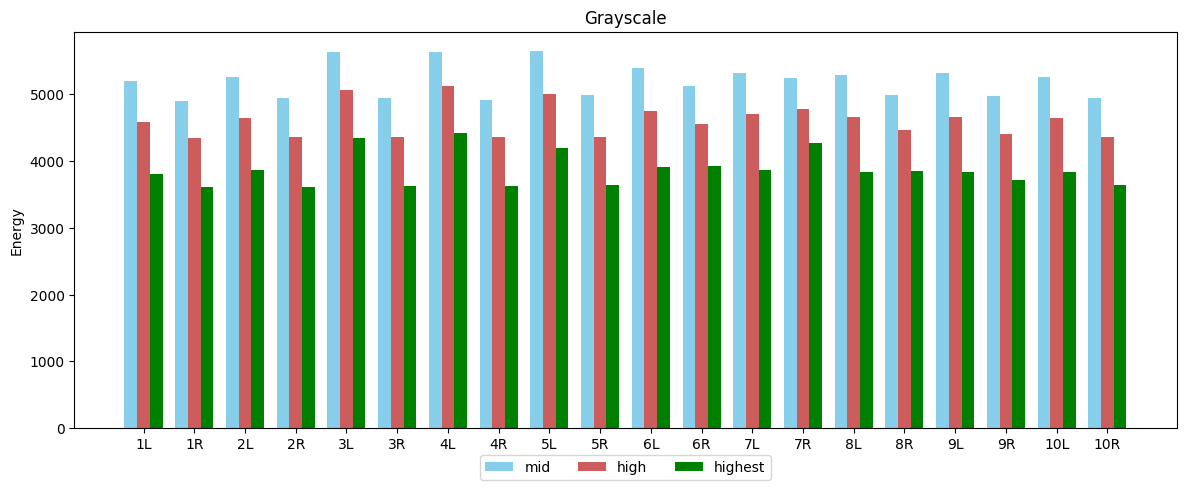
\includegraphics[scale=0.4]{images/appendix/stft/coin_o/hann_Grayscale.png}
        \caption{}
    \end{subfigure}\\
    \begin{subfigure}{\textwidth}
         \centering
          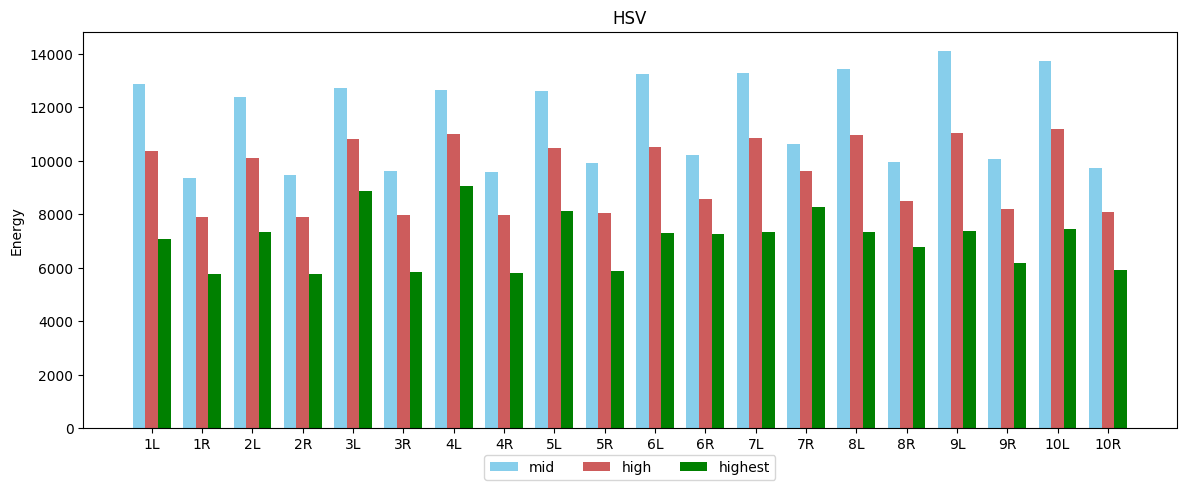
\includegraphics[scale=0.4]{images/appendix/stft/coin_o/hann_HSV.png}
          \caption{}
    \end{subfigure}
    \fautor
\end{figure}

\begin{figure}[H]
    \caption{Card STFT approach with Hann window for Grayscale (a) and HSV (b) colourspaces.}
    \centering
    \begin{subfigure}{\textwidth}
        \centering
        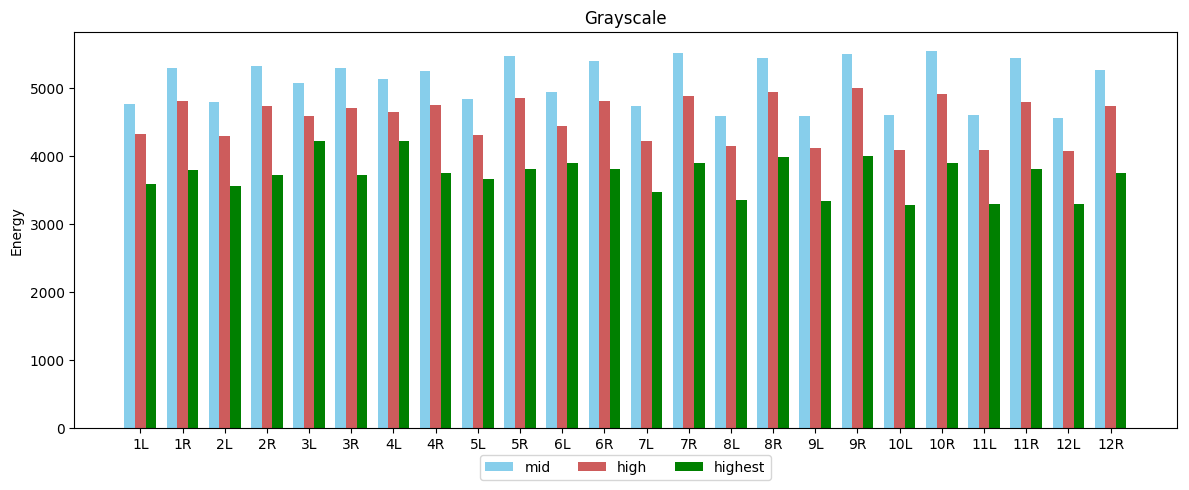
\includegraphics[scale=0.5]{images/appendix/stft/card/hann_Grayscale.png}
        \caption{}
    \end{subfigure}\\
    \begin{subfigure}{\textwidth}
         \centering
          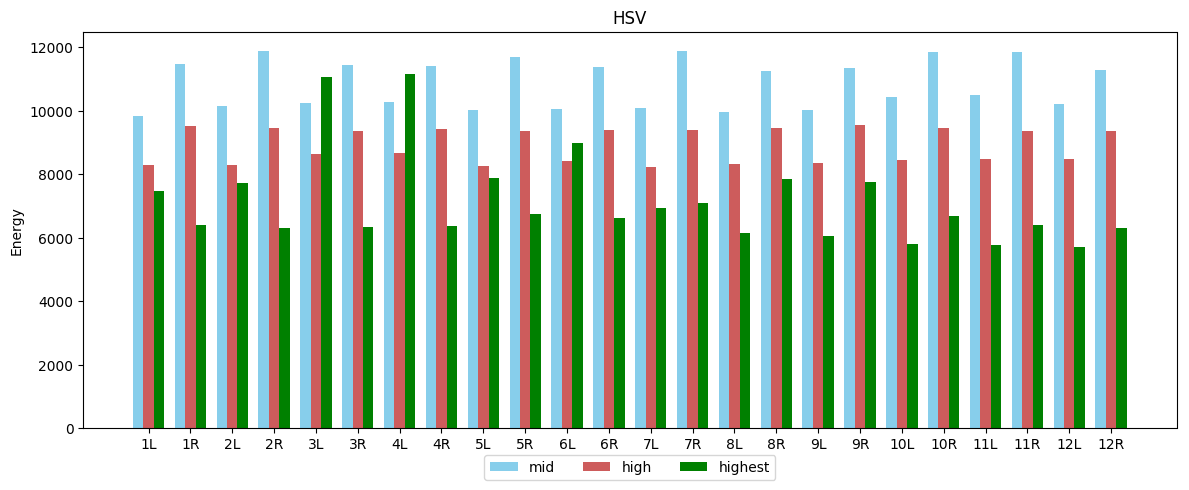
\includegraphics[scale=0.5]{images/appendix/stft/card/hann_HSV.png}
          \caption{}
    \end{subfigure}
    \fautor
\end{figure}

\begin{figure}[H]
    \caption{Airplane STFT approach with Hann window for Grayscale (a) and HSV (b) colourspaces.}
    \centering
    \begin{subfigure}{.5\textwidth}
        \centering
        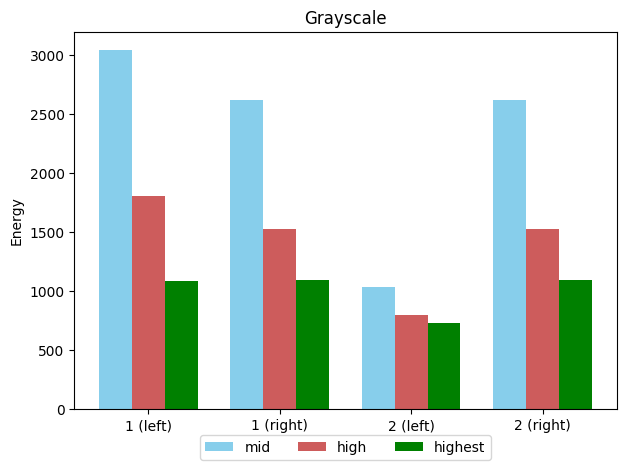
\includegraphics[scale=0.41]{images/appendix/stft/airplane/hann_Grayscale.png}
        \caption{}
    \end{subfigure}%
    \begin{subfigure}{.5\textwidth}
         \centering
          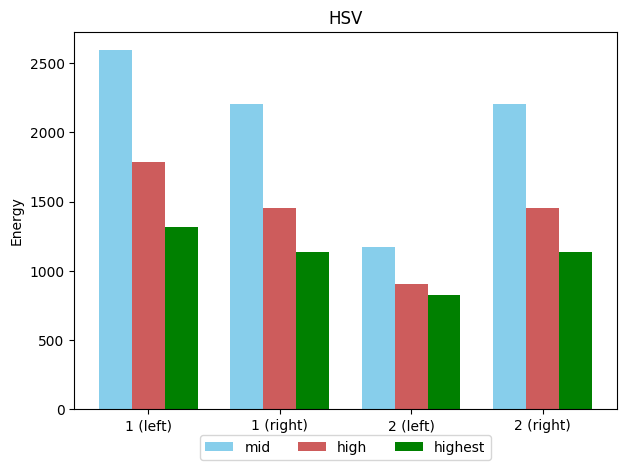
\includegraphics[scale=0.41]{images/appendix/stft/airplane/hann_HSV.png}
          \caption{}
    \end{subfigure}
    \fautor
\end{figure}


\begin{figure}[H]
    \caption{Coin "v" STFT approach with Hann window for Grayscale (a) and HSV (b) colourspaces.}
    \centering
    \begin{subfigure}{\textwidth}
        \centering
        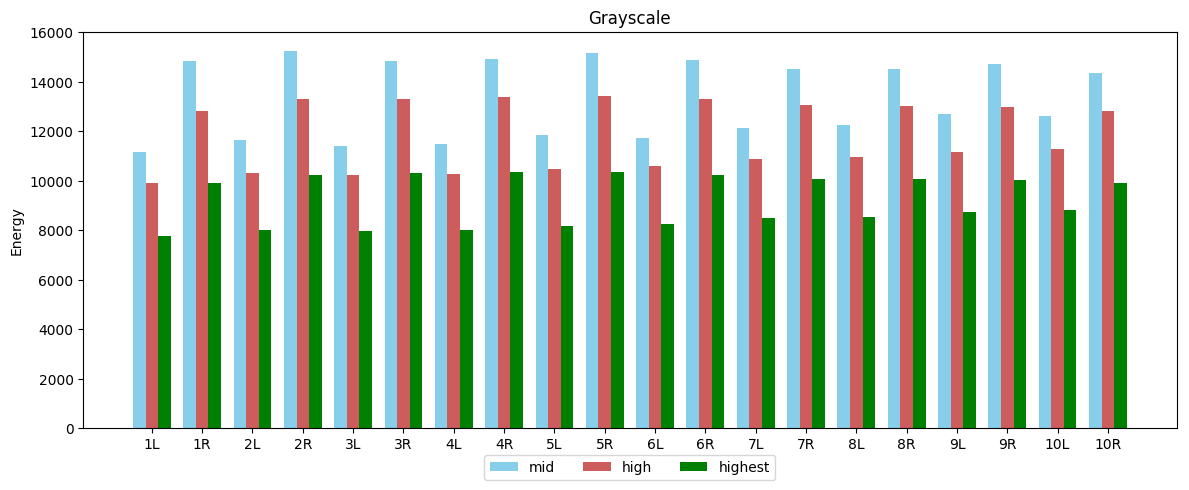
\includegraphics[scale=0.5]{images/appendix/stft/coin_v/hann_Grayscale.png}
        \caption{}
    \end{subfigure}\\
    \begin{subfigure}{\textwidth}
         \centering
          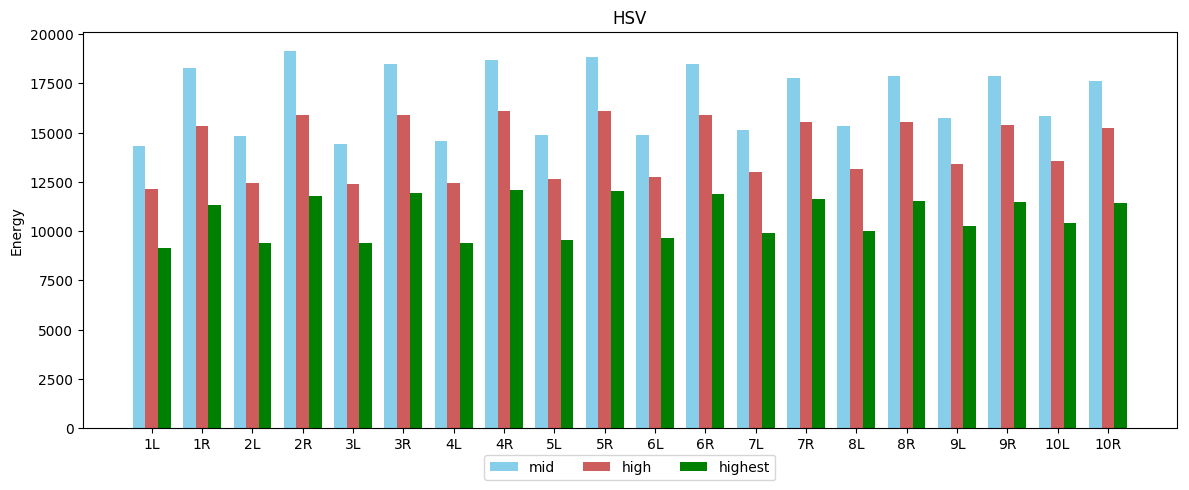
\includegraphics[scale=0.5]{images/appendix/stft/coin_v/hann_HSV.png}
          \caption{}
    \end{subfigure}
    \fautor
\end{figure}

\section{Flattop Window}

\begin{figure}[H]
    \caption{Airplane STFT approach with Flattop window for Grayscale (a) and HSV (b) colourspaces.}
    \centering
    \begin{subfigure}{.5\textwidth}
        \centering
        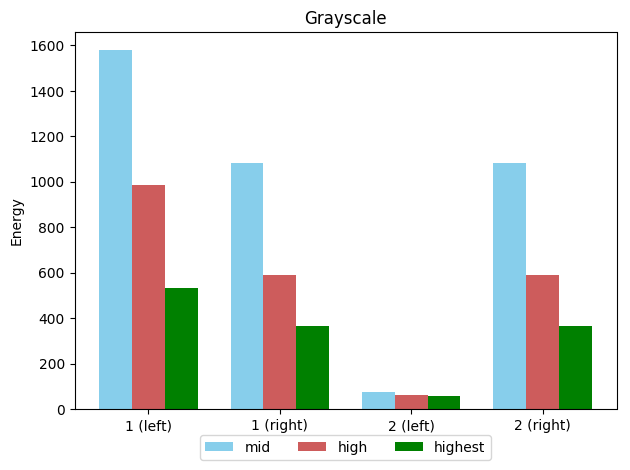
\includegraphics[scale=0.41]{images/appendix/stft/airplane/flattop_Grayscale.png}
        \caption{}
    \end{subfigure}%
    \begin{subfigure}{.5\textwidth}
         \centering
          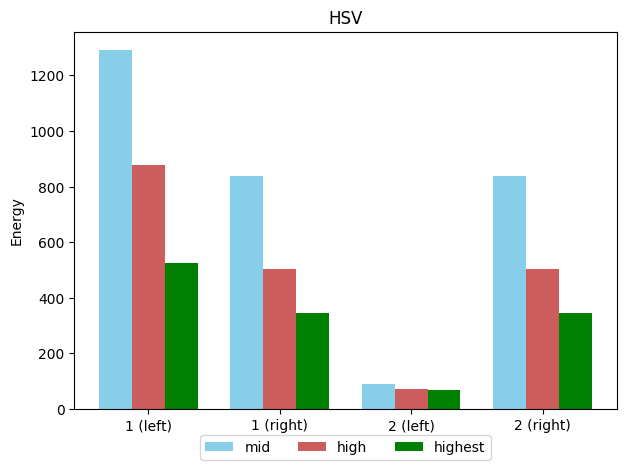
\includegraphics[scale=0.41]{images/appendix/stft/airplane/flattop_HSV.png}
          \caption{}
    \end{subfigure}
    \fautor
\end{figure}

\begin{figure}[!htb]
    \caption{Coin "o" STFT approach with Flattop window for Grayscale (a) and HSV (b) colourspaces.}
    \centering
    \begin{subfigure}{\textwidth}
        \centering
        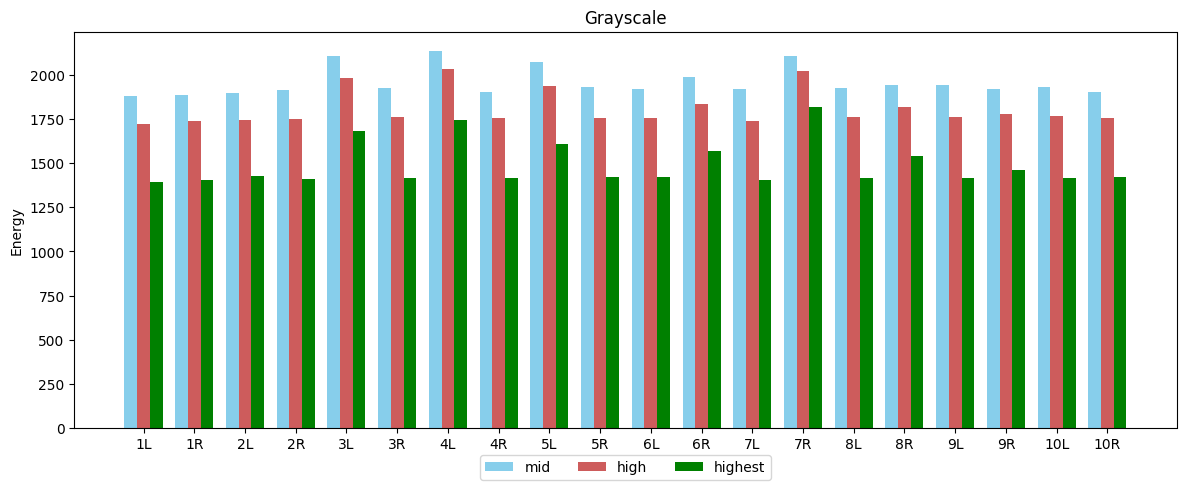
\includegraphics[scale=0.4]{images/appendix/stft/coin_o/flattop_Grayscale.png}
        \caption{}
    \end{subfigure}\\
    \begin{subfigure}{\textwidth}
         \centering
          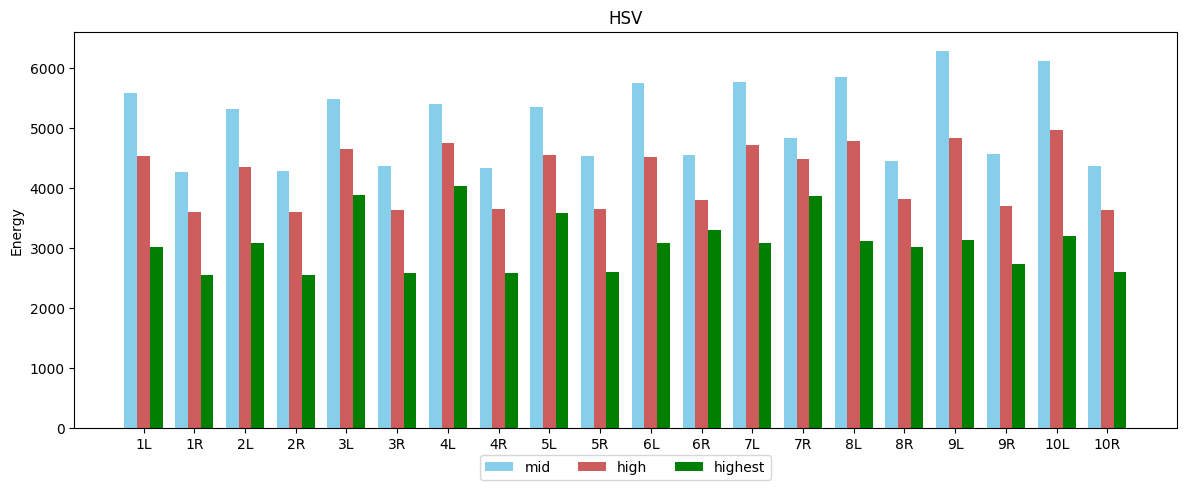
\includegraphics[scale=0.4]{images/appendix/stft/coin_o/flattop_HSV.png}
          \caption{}
    \end{subfigure}
    \fautor
\end{figure}

\begin{figure}[H]
    \caption{Card STFT approach with Flattop window for Grayscale (a) and HSV (b) colourspaces.}
    \centering
    \begin{subfigure}{\textwidth}
        \centering
        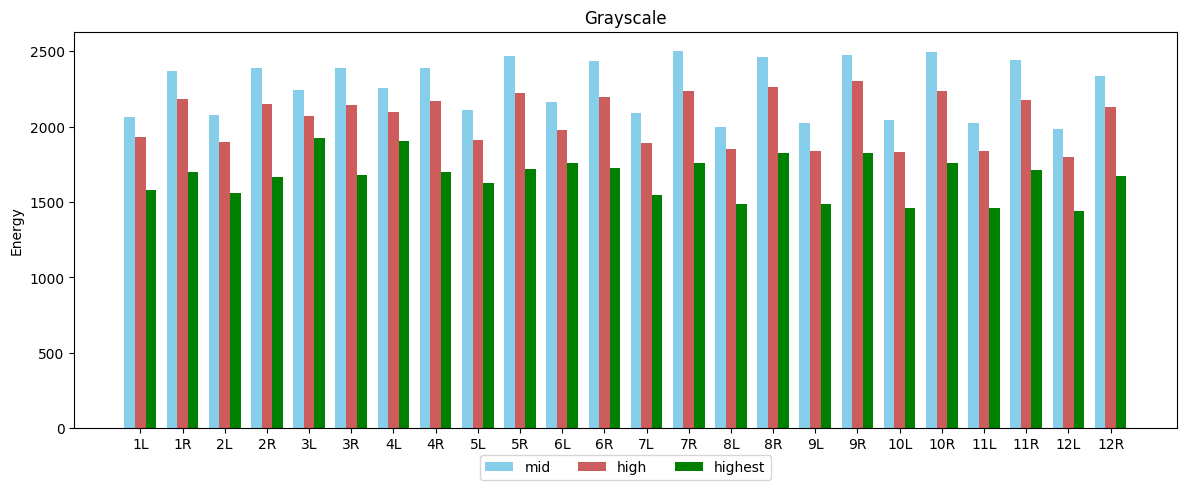
\includegraphics[scale=0.5]{images/appendix/stft/card/flattop_Grayscale.png}
        \caption{}
    \end{subfigure}\\
    \begin{subfigure}{\textwidth}
         \centering
          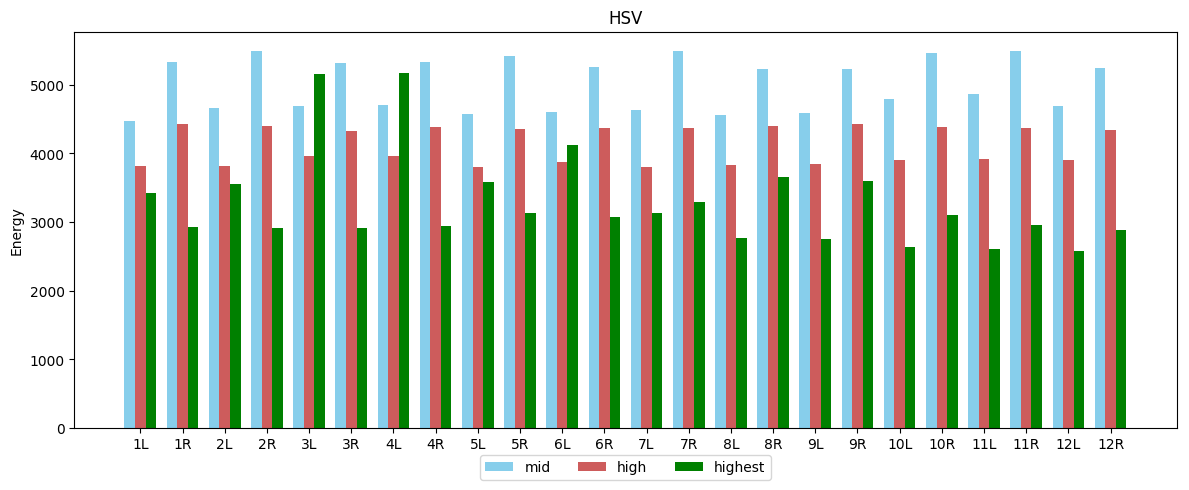
\includegraphics[scale=0.5]{images/appendix/stft/card/flattop_HSV.png}
          \caption{}
    \end{subfigure}
    \fautor
\end{figure}


\begin{figure}[H]
    \caption{Coin "v" STFT approach with Flattop window for Grayscale (a) and HSV (b) colourspaces.}
    \centering
    \begin{subfigure}{\textwidth}
        \centering
        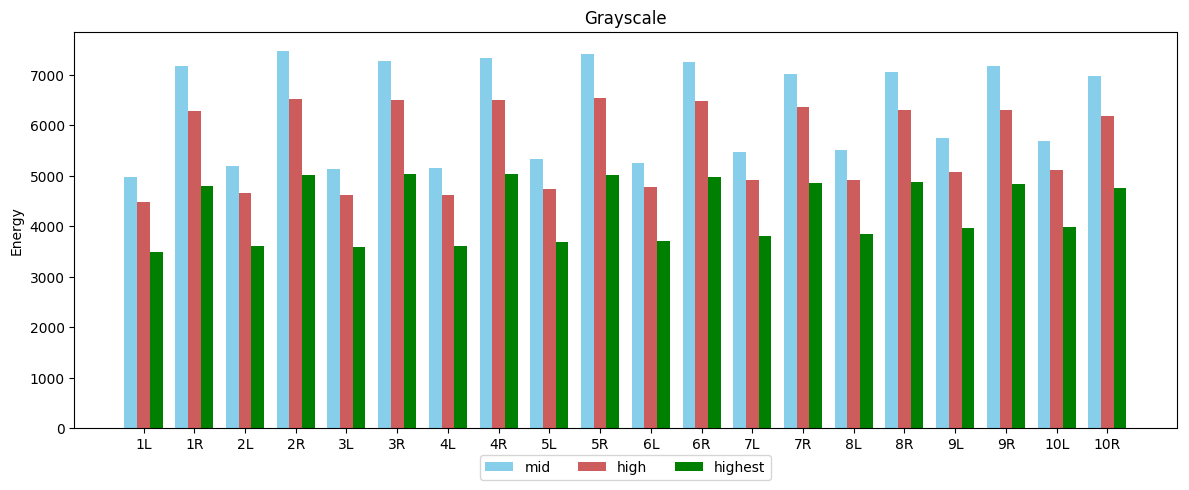
\includegraphics[scale=0.5]{images/appendix/stft/coin_v/flattop_Grayscale.png}
        \caption{}
    \end{subfigure}\\
    \begin{subfigure}{\textwidth}
         \centering
          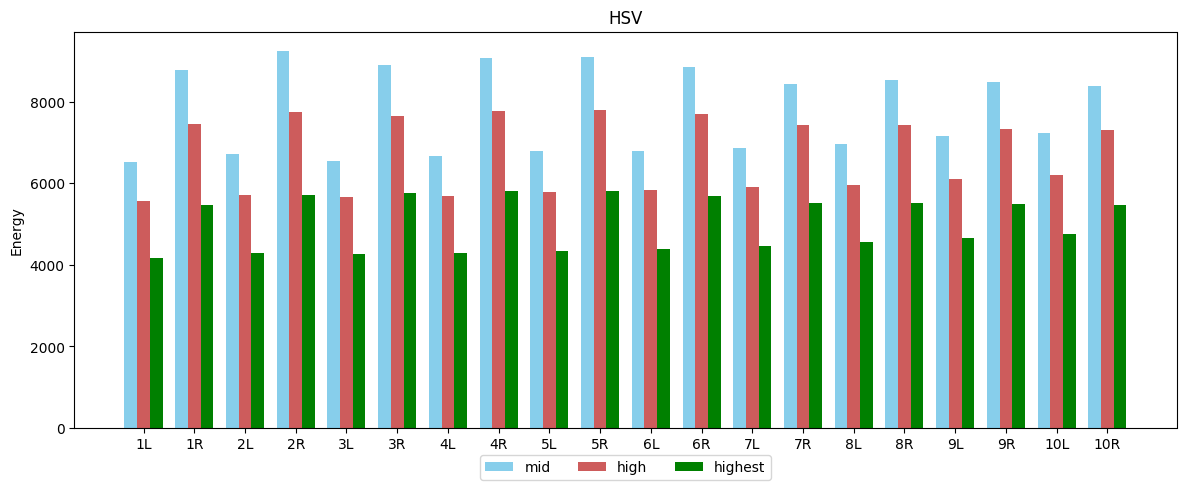
\includegraphics[scale=0.5]{images/appendix/stft/coin_v/flattop_HSV.png}
          \caption{}
    \end{subfigure}
    \fautor
\end{figure}

\section{Blackmanharris Window}

\begin{figure}[H]
    \caption{Airplane STFT approach with Blackmanharris window for Grayscale (a) and HSV (b) colourspaces.}
    \centering
    \begin{subfigure}{.5\textwidth}
        \centering
        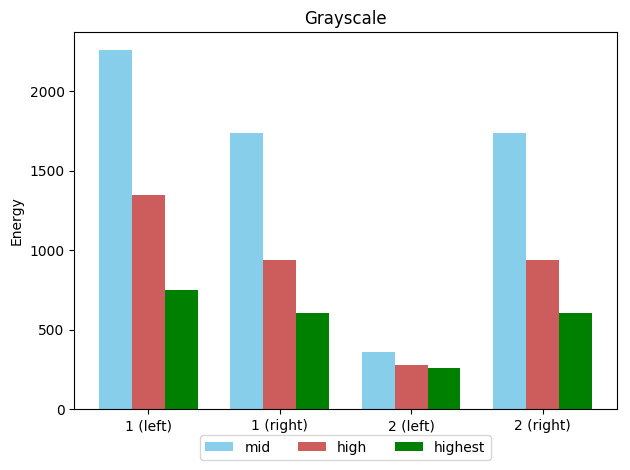
\includegraphics[scale=0.41]{images/appendix/stft/airplane/blackmanharris_Grayscale.png}
        \caption{}
    \end{subfigure}%
    \begin{subfigure}{.5\textwidth}
         \centering
          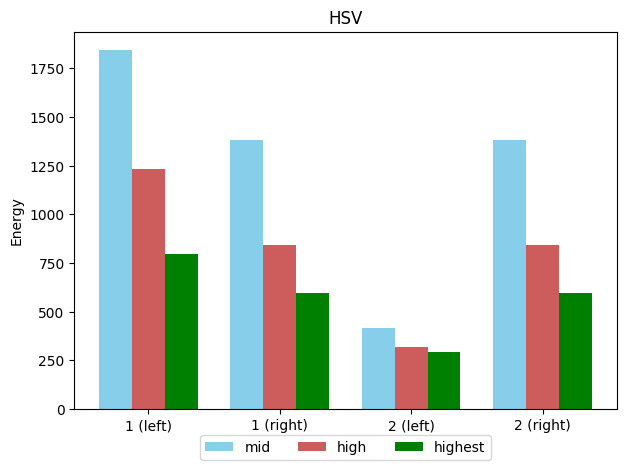
\includegraphics[scale=0.41]{images/appendix/stft/airplane/blackmanharris_HSV.png}
          \caption{}
    \end{subfigure}
    \fautor
\end{figure}

\begin{figure}[H]
    \caption{Coin "o" STFT approach with Blackmanharris window for Grayscale (a) and HSV (b) colourspaces.}
    \centering
    \begin{subfigure}{\textwidth}
        \centering
        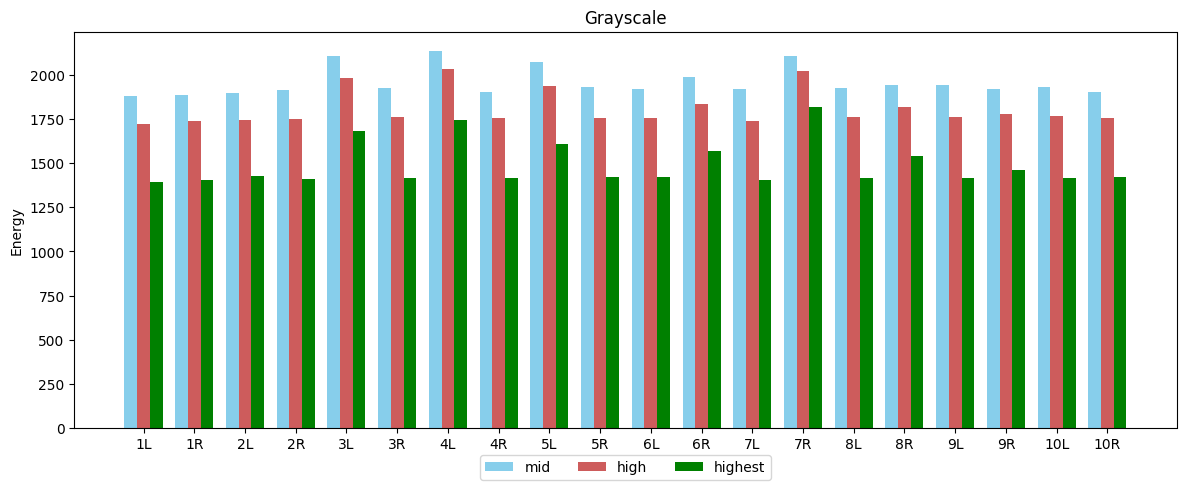
\includegraphics[scale=0.4]{images/appendix/stft/coin_o/flattop_Grayscale.png}
        \caption{}
    \end{subfigure}\\
    \begin{subfigure}{\textwidth}
         \centering
          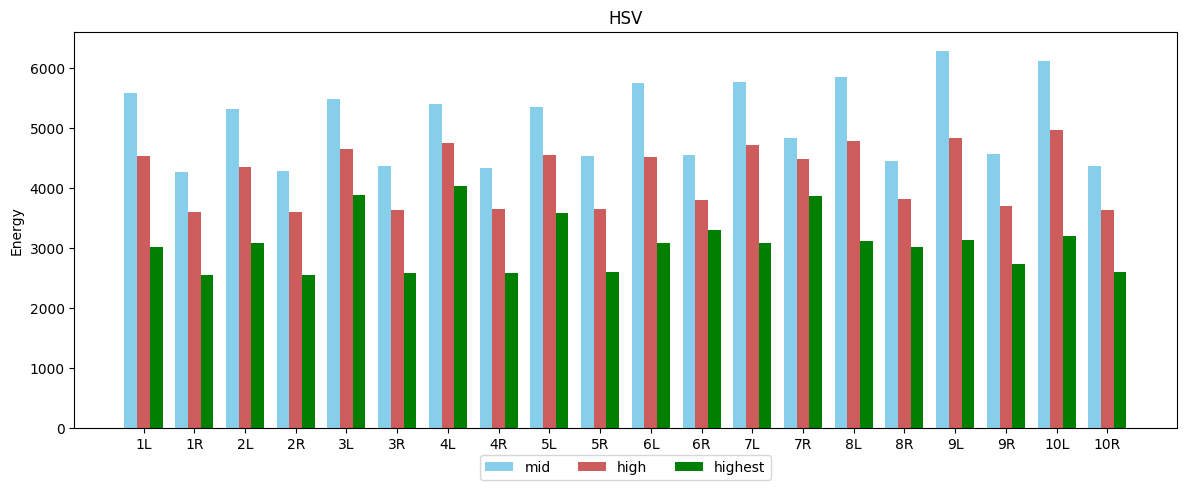
\includegraphics[scale=0.4]{images/appendix/stft/coin_o/flattop_HSV.png}
          \caption{}
    \end{subfigure}
    \fautor
\end{figure}

\begin{figure}[H]
    \caption{Card STFT approach with Blackmanharris window for Grayscale (a) and HSV (b) colourspaces.}
    \centering
    \begin{subfigure}{\textwidth}
        \centering
        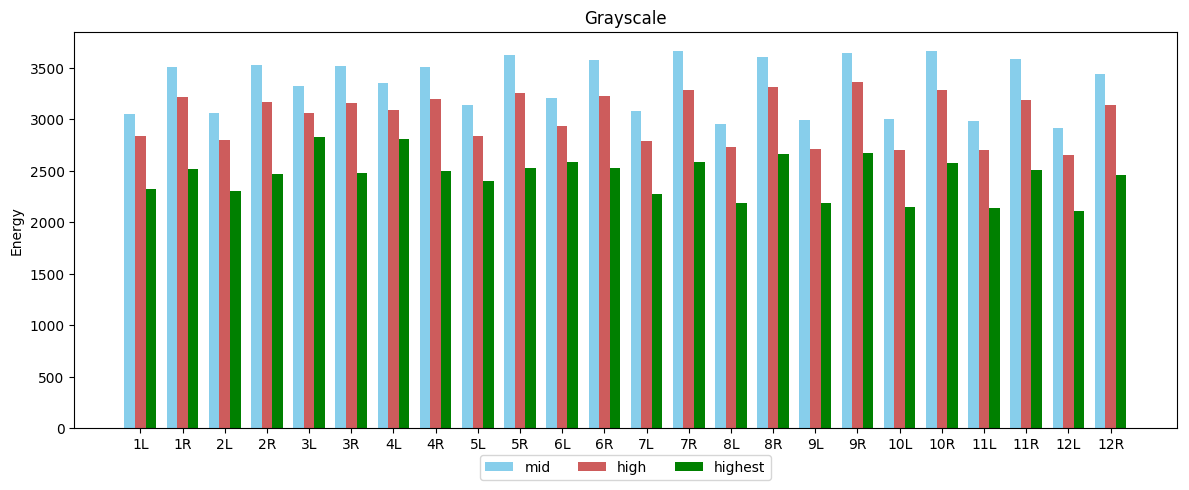
\includegraphics[scale=0.5]{images/appendix/stft/card/blackmanharris_Grayscale.png}
        \caption{}
    \end{subfigure}\\
    \begin{subfigure}{\textwidth}
         \centering
          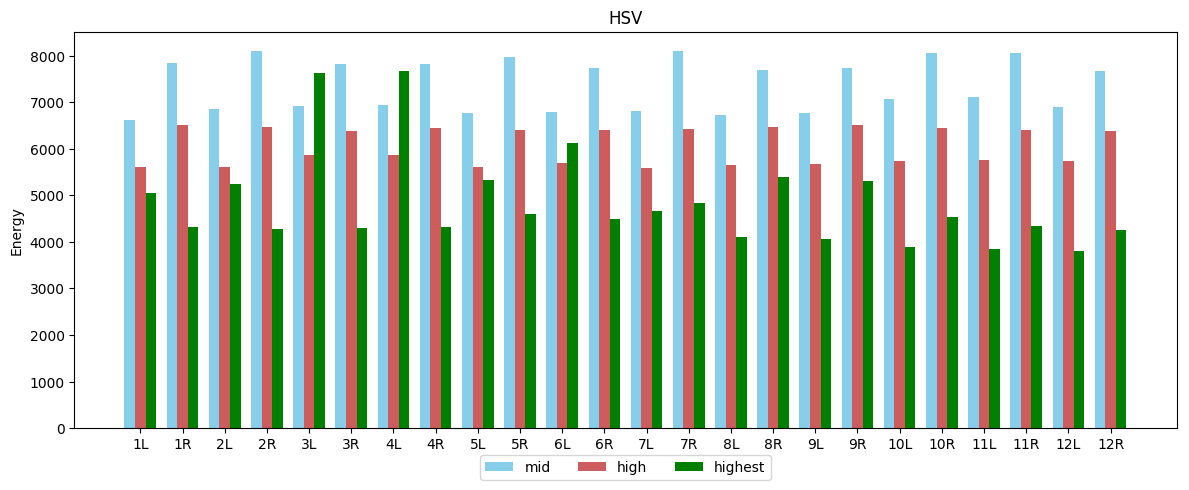
\includegraphics[scale=0.5]{images/appendix/stft/card/blackmanharris_HSV.png}
          \caption{}
    \end{subfigure}
    \fautor
\end{figure}

\begin{figure}[H]
    \caption{Coin "v" STFT approach with Blackmanharris window for Grayscale (a) and HSV (b) colourspaces.}
    \centering
    \begin{subfigure}{\textwidth}
        \centering
        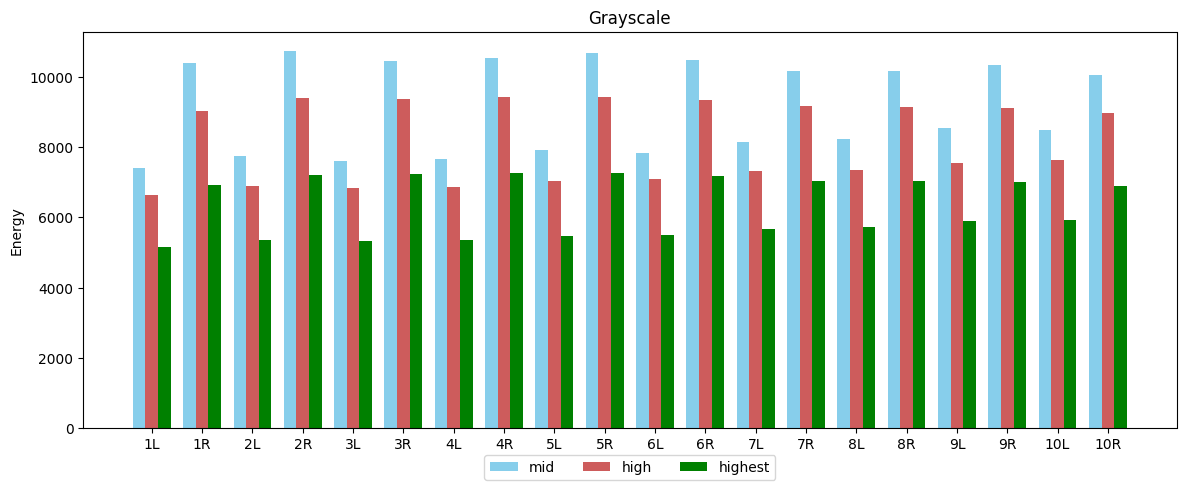
\includegraphics[scale=0.5]{images/appendix/stft/coin_v/blackmanharris_Grayscale.png}
        \caption{}
    \end{subfigure}\\
    \begin{subfigure}{\textwidth}
         \centering
          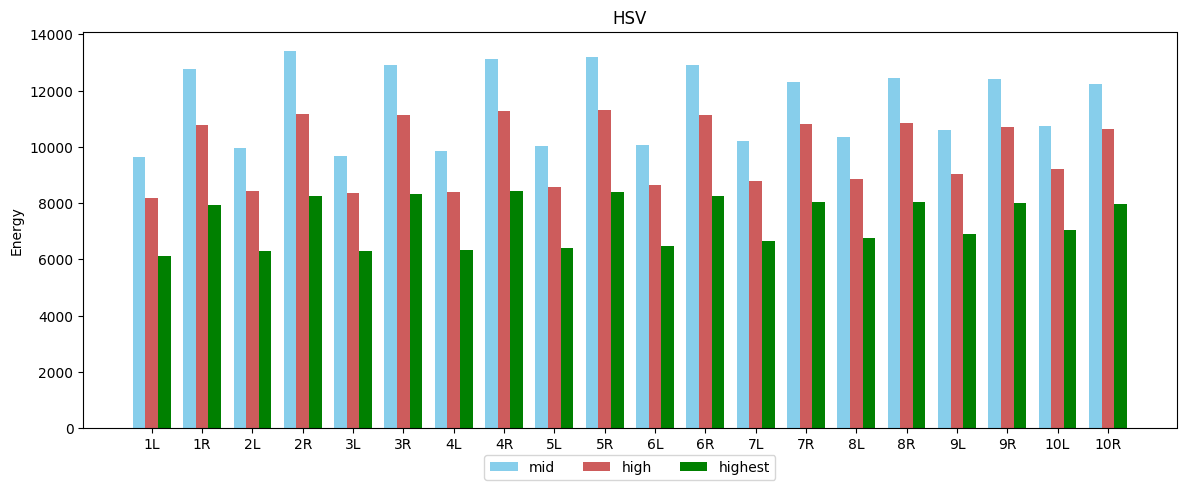
\includegraphics[scale=0.5]{images/appendix/stft/coin_v/blackmanharris_HSV.png}
          \caption{}
    \end{subfigure}
    \fautor
\end{figure}